\documentclass[../../dissertation.tex]{subfiles}
\begin{document}

As was seen in section \ref{sec:chap3Contwalk}, the unitary evolution operator of this model is defined as
\begin{equation}
        U(t) = e^{-iHt} = e^{i(-\gamma L)t} = e^{-i\gamma(A+D)t}.
\end{equation}
Considering a regular graph, this operator can be rewritten as 
\begin{equation}
	U(t) = \phi(t) e^{-i\gamma(A)t},
\end{equation}
where $\phi(t)$ is a global phase and $A$ is the adjacency matrix associated with the graph.\par
Here, the study will focus on the circuit implementation of this walk in a cyclic graph, and a different approach was used to define the adjacency matrix. This approach relies on the concept of a circulant graph, which are a class of graphs defined by a circulanti matrix such that
\begin{equation}
A = 
	\begin{pmatrix}
		c_0&c_{N-1}& \cdots&c_3&c_2 \\
		c_1&c_0& c_{N-1}& &c_{3} \\
		\vdots & c_1 & c_0 &\ddots & \vdots\\
		c_{N-2}& & \ddots&\ddots &c_{N-1}\\
		c_{N-1} & c_{N-2} & \cdots & c_1 & c_0\\
	\end{pmatrix}.
\label{eq:adjCirculant}
\end{equation}
In order to generate the proper circulant graphs, restrictions on this matrix are needed. Firstly, $c_0=0$, since self-loops are not part of the structure. Secondly, the matrix must be symmetric, therefore $c_{n-j} = c_j$.\par
These matrices can be fully described by the first column of the matrix 
\begin{equation}
	v_1 = [c_{0},c_{1}, \cdots, c_{N-2}, c_{N-1}]^T 
\end{equation}
with a discrete convolution operator performing cyclic permutations of $c$, on each column. For example,
\begin{equation}
	D v_1 = [c_{N-1}, c_{0}, \cdots, c_{N-3}, c_{N-2}]^T = v_2.
\end{equation}
More specifically, for the cycle case
\begin{equation}
	D v_1 = D [0, 1 ,0 , \cdots, 0, 1]^T =[1, 0, 1, 0, \cdots, 0, 0]^T = v_2.
\end{equation}
%TODO: Estas definicoes estao mal. 
The operator can then be recursively defined as
\begin{equation}
    Dv_k = v_{k+1}.
\end{equation}
and the matrix will be
\begin{equation}
	A = \sum_{j=0}^{N-1} D v_j 
\end{equation}
\begin{equation}
	A^k = \sum_{j=0}^{N-1} c_{(j-1)\mod{N}}
\end{equation}\par
The eigenvalues of a circulant matrix can be found by
\begin{equation}
\lambda_p = c_0 + \sum_{q=1} c_{N-q} \omega^{pq},
\end{equation}
and the eigenvectors are 
\begin{equation}
\ket{\varphi_p} = \frac{1}{\sqrt{n}} \sum_{q=0}^{n-1} \omega^{pq}.
\end{equation}
This given, it is possible to construct an operator that diagonalizes the circulant matrix through the eigenvectors, which is useful for constructing the circuit. For this purpous, the Quantum Fourier Transform can be used and it is defined as 
\begin{equation}
F = \frac{1}{\sqrt{N}} \sum_{p,q} \omega^{pq} \ket{p}\bra{q}.
\end{equation}
The adjacency matrix of a circulant graph can then be diagonalized such that
\begin{equation}
    A = F^{\dagger} \Lambda F,
    \label{eq:qiskitContQWAdj}
\end{equation}
where $\Lambda$ is a diagonal operator that encodes the eigenvalues
\begin{equation}
\Lambda = \sum_{j} \lambda_j \ket{j}\bra{j}.
\end{equation}\par
%TODO: Mostrar o raciocinio da algebra.
The unitary operator of the walk can then be rewritten as
\begin{equation}\label{eq:diagUniOpCont}
    U = F^{\dagger}e^{i\gamma \Lambda t} F
\end{equation}
where
\begin{equation}
    e^{i\gamma \Lambda t} = \sum_{j} e^{i\gamma \lambda_j t} \ket{j}\bra{j}.
\end{equation}\par
%TODO: Explicar a diagonal()?
The circuit can now be constructed making use of the \textit{diagonal} function provided by Qiskit, which decomposes diagonal operators based on the method presented in theorem 7 of \cite{Shende06}. The other tool used was the Quantum Fourier Transform, also provided by the Qiskit package. Figure \ref{fig:contQWCircuitQistkit} shows the implementation of the circuit for 3 qubits or $2^3=8$ graph nodes and $t=3$.

\begin{figure}[!h]
	\centering
	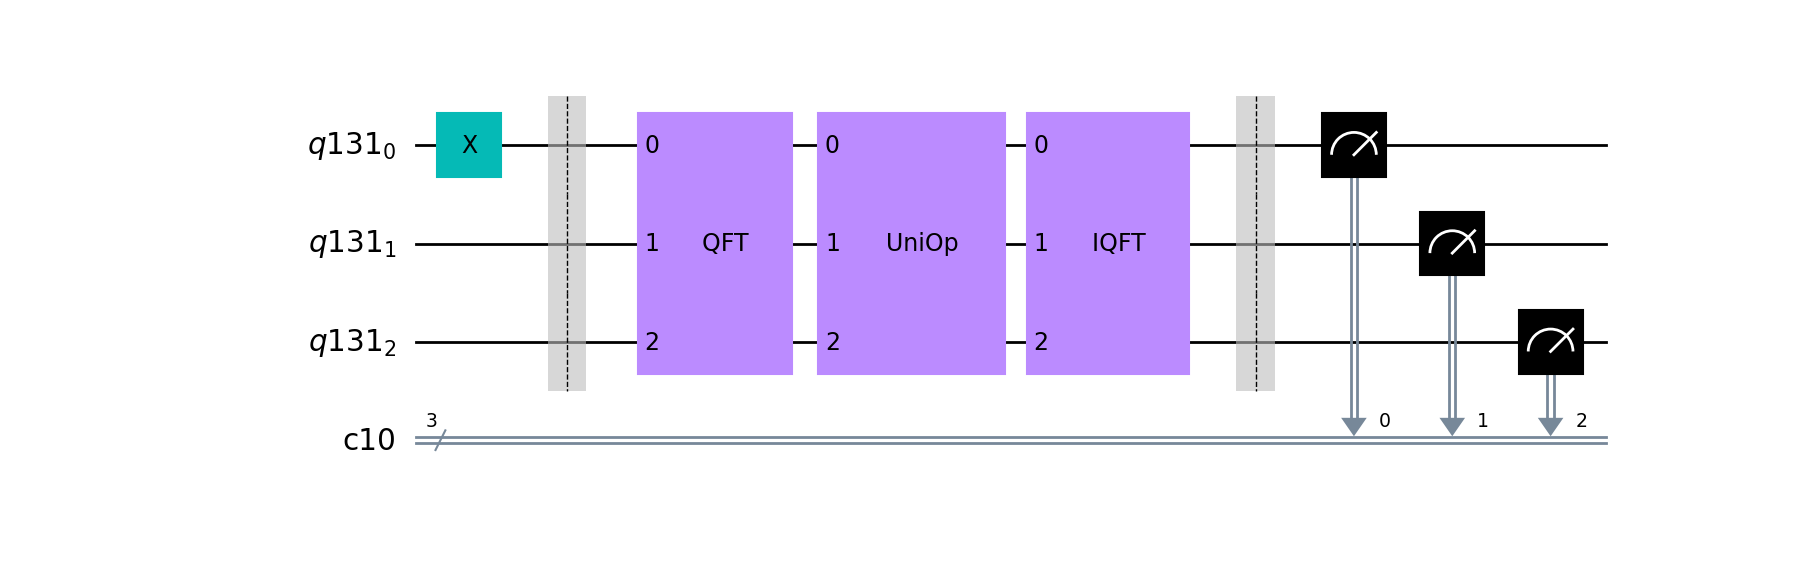
\includegraphics[scale=0.30]{img/Qiskit/ContQuantumWalk/Circuits/circContQW_N3_S1.png}
	\caption{Temp} 
	\label{fig:contQWCircuitQistkit}
\end{figure}
%TODO: Perceber como explicar a QFT.
The circuit for the Quantum Fourier transform is well known and presented in figure \ref{fig:qftCircuitQiskit}. The circuit associated with $F^{\dagger}$ is similarly constructed by negating the previous figure's rotations.\par
\begin{figure}[!h]
	\centering
	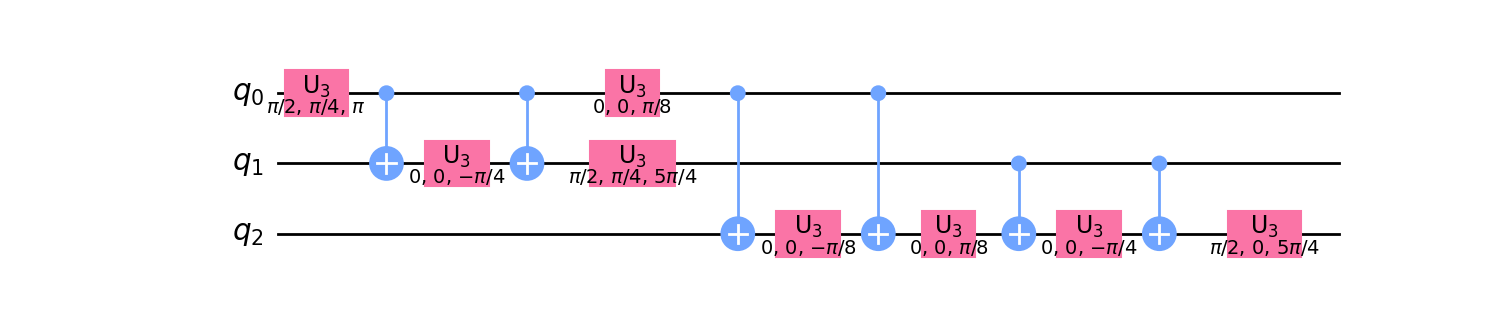
\includegraphics[scale=0.30]{img/Qiskit/ContQuantumWalk/Circuits/circQft_N3_S1.png}
	\caption{Temp} 
	\label{fig:qftCircuitQiskit}
\end{figure}
The circuit associated with the diagonal operator is show in figure \ref{fig:diagCircuitQiskit}. Furthermore equation \ref{eq:diagUniOpCont} says that time is simply a constant inside the exponential, which means that the diagonal operator's circuit will not need extra gates when increasing time, it will only need different rotations and differ in global phase. 
\begin{figure}[!h]
	\centering
	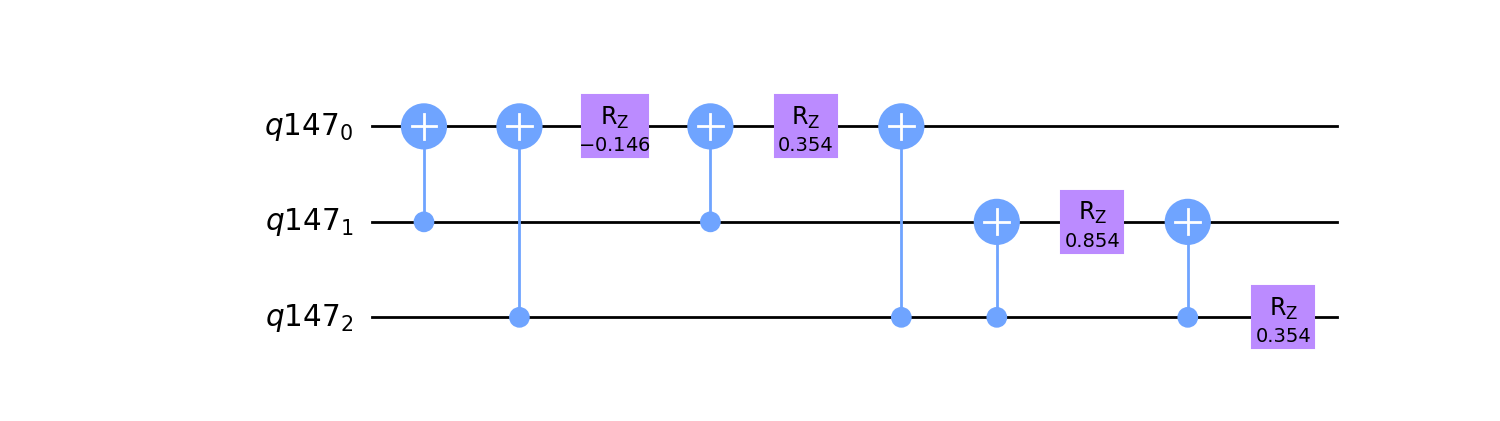
\includegraphics[scale=0.30]{img/Qiskit/ContQuantumWalk/Circuits/circDiag_N3_S1.png}
	\caption{temp}
	\label{fig:diagCircuitQiskit}
\end{figure}
This is an advantage when comparing to the previous model, seen in figure \ref{fig:coinedQWCircuitQistkit}, where each extra step required another increment and decrement gates.  Further evidence of this behaviour can be seen in figure \ref{fig:gateCountQiskit}, where it was created a circuit for $t=0$ up to $t=100$ with increments of $1$. It was then counted the number of gates, for each circuit, and plotted against the respective time. 
\begin{figure}[!h]
	\centering
	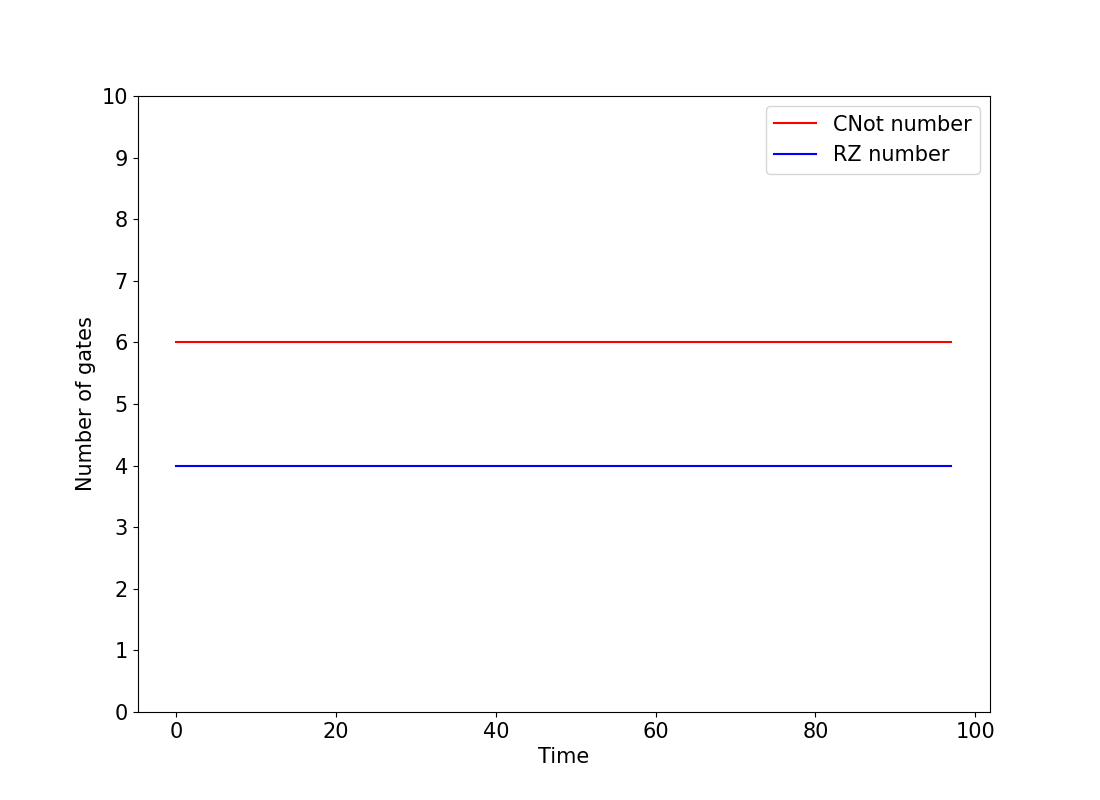
\includegraphics[scale=0.35]{img/Qiskit/ContQuantumWalk/gateCount_N3.png}
	\caption{Temp} 
	\label{fig:gateCountQiskit}
\end{figure}
%TODO: Acabar analise de resultados!!
This graph clearly shows that both the number of $R_z$ rotations and CNot operations remain constant throughout the entire time interval.\par
Finally, the circuit was measured, and the result can be seen in figure \ref{fig:contQWQiskitDist} 
\begin{figure}[!h]
	\centering
	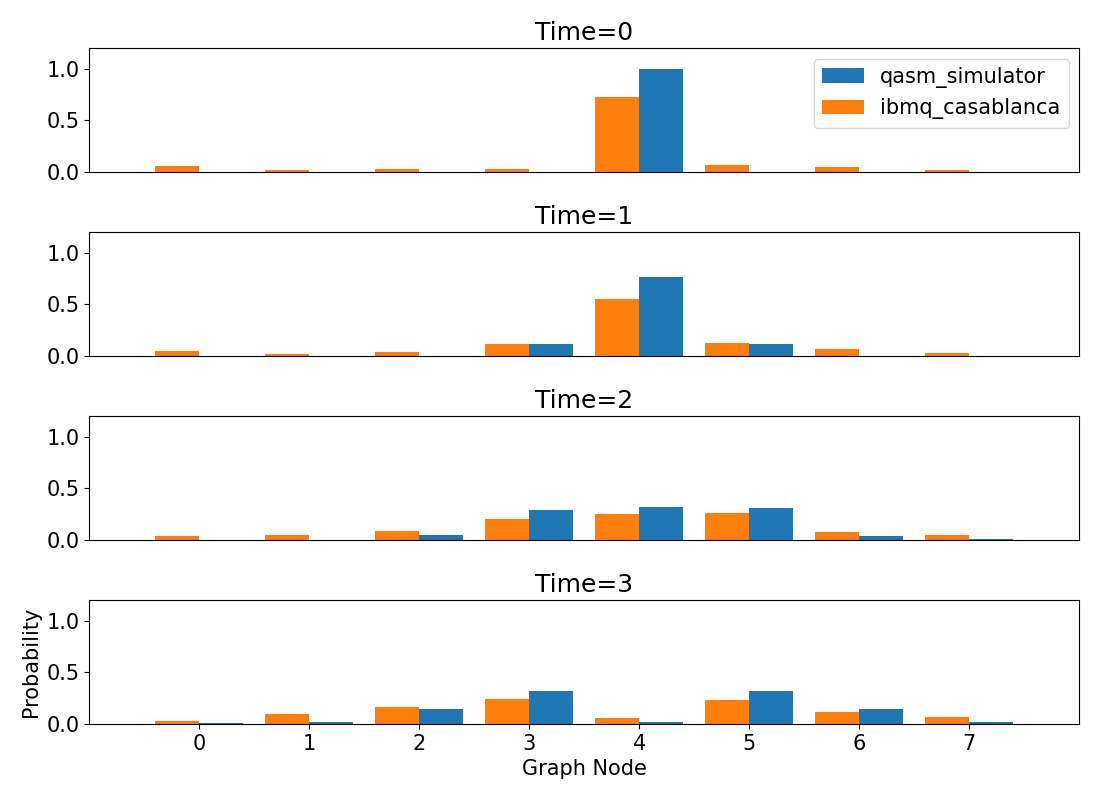
\includegraphics[scale=0.35]{img/Qiskit/ContQuantumWalk/ContQW_N3_S0123.png}
	\caption{Temp} 
	\label{fig:contQWQiskitDist}
\end{figure}

\end{document}
